\documentclass[a4paper]{article}
\usepackage[utf8]{inputenc}
\usepackage[a4paper, left=2.5cm, right=2.5cm, top=2cm, bottom=2cm]{geometry}
\usepackage{lmodern}
\usepackage[T1]{fontenc}
\usepackage{graphicx}
\usepackage{amssymb}
\usepackage[utf8]{inputenc}
\usepackage{pgfplots}
\pgfplotsset{width=8cm,compat=1.9}
\usepackage{multicol}
\usepackage{csquotes}
\usepackage{amsfonts}
\usetikzlibrary{angles, quotes}

\newcommand{\overbar}[1]{\mkern 1.5mu\overline{\mkern-1.5mu#1\mkern-1.5mu}\mkern 1.5mu}
\renewcommand{\thesection}{\Alph{section}}
\renewcommand{\thesubsection}{\arabic{subsection}}
\renewcommand{\thesubsubsection}{(\emph{\alph{subsubsection}})}

\title{Ondes et particules}
\author{Hugo Lageneste}
\date{Février 2020}

\begin{document}

{Hugo \textsc{Lageneste}}\\
{Physique-Chimie - Ondes et particules}

\begin{center}
 \newcommand{\HRule}{\rule{\linewidth}{0.5mm}}
 {\huge \bfseries Ondes et particules}\\[0.1cm]
\end{center}

\section{Caractérisation des ondes}
\subsection{Direction de la perturbation}
{Une onde se propage longitudinalement lorsque la perturbation se fait parallèlement à la direction de propagation}\\
{Une onde se propage transversalement lorsque la perturbation se fait perpendiculairement à la direction de propagation}

\subsection{Période et fréquence}
{La période $T$ est la durée pour qu'un point revienne dans un même état vibratoire}
\begin{center}
	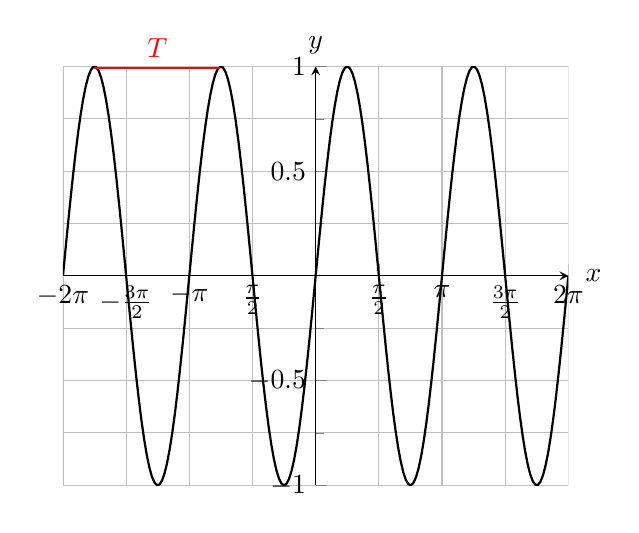
\begin{tikzpicture}
       	\pgfmathdeclarefunction{S}{2}{\pgfmathparse{sin(deg(#1*#2))}}
      	\begin{axis}[
    xtick={
        -6.28318, -4.7123889, -3.14159, -1.5708,
        1.5708, 3.14159, 4.7123889, 6.28318
    },
    xticklabels={
        $-2\pi$, $-\frac{3\pi}{2}$, $-\pi$, $\frac{\pi}{2}$,
        $\frac{\pi}{2}$, $\pi$, $\frac{3\pi}{2}$, $2\pi$
    },
    axis lines = center,
    grid=both,minor tick num=1,
    xlabel=$x$,ylabel=$y$,
    tick align=inside,
        legend style={at={(0.5,-0.1)},
        anchor=north,legend columns=2},
        domain=-2*pi:2*pi,
        samples=200,
        every axis y label/.style={rotate=0, black, at={(0.5,1.05)},},
        every axis x label/.style={rotate=0, black, at={(1.05,0.5)},},
        ]
        \addplot [thick] {S(2,x)};
       \end{axis}
        \draw[red,thick]  (0.4,5.3) to ["$T$"] (2,5.3);
	\end{tikzpicture}\\
\end{figure}
{La fréquence $F$ (en Hz) représente le nombre de répétitions de la perturbation par secondes.}\\
{On peut l'exprimer en fonction de la période $T$}
\[F=\frac{1}{T}\]

\subsection{Longueur d'onde}
{La longueur d'onde $\lambda$ est la distance pour qu'un point revienne dans un même état vibratoire}\\
{On peut lier la longueur d'onde, la célérité et la période d'une onde avec cette formule:}
\[c=\frac{\lambda}{T}\quad\Leftrightarrow\quad c=\lambda \times F\]


\end{document}